\chapter{Аналитический раздел}
В данном разделе представлено описание 3D-сцены, а также рассмотрены алгоритмы визуализации сцены и генерации ландшафта.

\section{Формализация объектов сцены}
Сцена состоит из следующих объектов:
\begin{itemize}
	\item ландшафт — представлен трехмерной моделью. Предусмотрено задание характеристик ландшафта для изменения вида. Доступны настройки изменения размера (длина, ширина);
	\item источник света — представляет собой материальную точку, которая испускает лучи света.
\end{itemize}

\section{Представление данных о ландшафте}
В настоящее время существует несколько основных принципов представления данных для хранения информации о ландшафте \cite{data_landscape}.
\begin{enumerate}
	\item Использование регулярной сетки высот (карта высот).
	\item Использование иррегулярной сетки высот (хранение триангулированной карты).
	\item Посегментная карта высот.
\end{enumerate}

Рассмотрим более детально первые два способа.
\subsection{Регулярная сетка высот}
Модель равномерной сетки описывает координаты отдельных точек поверхности следующим образом: каждому узлу сетки с индексами $(i,j)$ приписывается значение высоты $z_{ij}$ (рисунок \ref{png:regular_height_grid}).

\begin{figure}[H]
	\centering{
		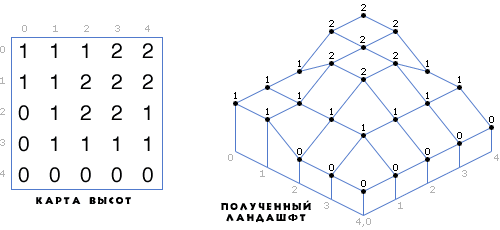
\includegraphics[scale=0.8]{../../../../../../../msys64/home/Лев/bmstu_cg_course_project/rpz/images/regular_height_grid}
		\caption{Регулярная сетка высот}
		\label{png:regular_height_grid}
	}
\end{figure}

Индексам $(i,j)$ соответствуют значения координат $(x, у)$ точки. Расстояние между узлами одинаковое $dx$ по оси $OX$, $dу$ по оси $OY$. Фактически такая модель - это матрица, каждый элемент которой сохраняет значение высоты $z$.

При помощи равномерной сетки высот часто описывают рельеф земной поверхности, так как такой подход имеет ряд преимуществ.
\begin{itemize}
	\item Довольно просто описывается поверхность, легкая модификация данных.
	\item Легкость нахождения координат и их высот.
	\item Можно производить динамическое освещение ввиду того, что вершинные точки расположены равномерно и близко друг к другу.
	\item Наглядность - карту высот можно хранить в графическом виде.
	\item Промежуточные значения можно вычислить путем интерполяции значений в вершинах сетки.
\end{itemize}

Недостатки:
\begin{itemize}
	\item при таком подходе невозможно описать все виды поверхностей, так как здесь используется для каждой координаты $x, y$ единственное значение z (то есть получаем функцию $z = f(x, y)$). Это является той поверхностью, которую каждая вертикаль пересекает только один раз;
	\item для описания сложных поверхностей требуется большее число узлов.
\end{itemize}

\subsection{Иррегулярная сетка вершин и их соединяющих}
Неравномерной сеткой называется модель описания поверхности в виде множества отдельных точек ${(x_{0}, y_{0}, z_{0}), (x_{1}, y_{1}, z_{1}), ... (x_{n-1}, y_{n-1}, z_{n-1})}$, принадлежащих ей. Эти точки могут быть получены, например, в результате измерений поверхности какого-нибудь объекта с помощью определенного оборудования. Равномерная сетка могут считается разновидностью неравномерной сетки вершин.

Рассмотрим модель поверхности в виде множества точечных значений, логически никак не связанных между собой (рисунок \ref{png:irregular_height_grid}). 
\begin{figure}[H]
	\centering{
		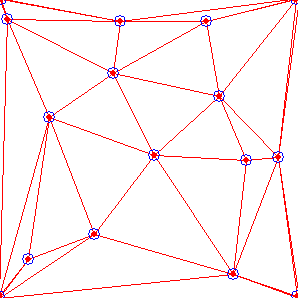
\includegraphics[scale=0.6]{../../../../../../../msys64/home/Лев/bmstu_cg_course_project/rpz/images/irregular_height_grid}
		\caption{Иррегулярная сетка высот}
		\label{png:irregular_height_grid}
	}
\end{figure}

Неравномерность задания опорных точек усложняет определение координат для других точек поверхности, которые не совпадают с опорными точками. Требуются специальные методы пространственной интерполяции.

Выделяют следующие положительные черты такого подхода:
\begin{itemize}
	\item использование отдельных опорных точек, наиболее важных для заданной формы поверхности (имеет меньший объем информации по сравнению с другими моделями, например с равномерной сеткой);
	\item применение изолиний на картах и планах позволяет наглядно отображать рельеф поверхности.
\end{itemize}

Но у такого метода содержатся существенные недостатки:
\begin{itemize}
	\item невозможность или сложность выполнения многих операций над поверхностями;
	\item возникновение сложностей при динамическом освещении — вершины расположены достаточно далеко друг от друга и неравномерно.
\end{itemize}

\section{Алгоритм генерации карты высот, использующий шум Перлина}
Возникает проблема — как же получить эту карту высот. Для этого разработан алгоритм, который прост в понимании и являющийся некой базой для дальнейшей модификации и получении интересного результата — использование шума. Сам шум представляет собой набор чисел. Значение шума связывают с высотой. Таким образом, получаем карту высот. 
Первый революционный алгоритм, нашедший широкое применение в компьютерной графике, основан на шуме Перлина \cite{perlin_noise}. Шум Перлина - это функция генерации когерентного шума в пространстве (рисунок \ref{png:perlin_noise}). 

\begin{figure}[H]
	\centering{
		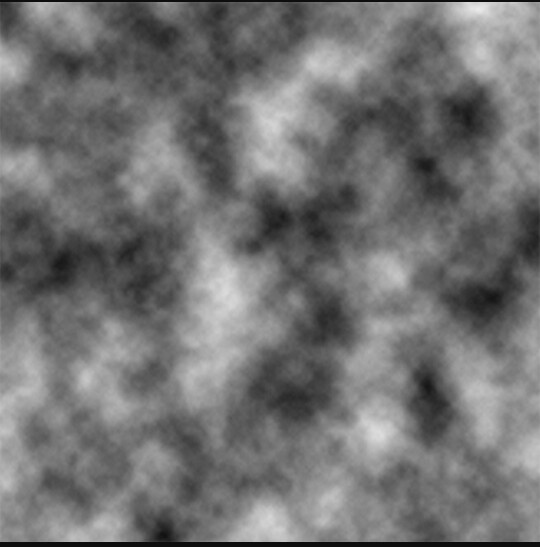
\includegraphics[scale=0.4]{../../../../../../../msys64/home/Лев/bmstu_cg_course_project/rpz/images/perlin_noise}
		\caption{Шум Перлина}
		\label{png:perlin_noise}
	}
\end{figure}

Кен Перлин предложил использовать вместо случайных значений в углах ячейки градиентный шум. Данный алгоритм может быть реализован для n-мерного пространства, но чаще всего реализуется для двух-, трех- или четырехмерного. 
Визуализация осуществляется как восьмиразрядные изображения с градациями серого, где каждая точка хранит высоту ландшафта в соответствующей позиции. Значения этой карты варьируются в диапазоне от 0 до 255, где 0 представляет самую низкую высоту вершины (на карте отображается как черный цвет), а 255 - максимально возможную (белый цвет). Этот интервал можно расширить, используя коэффициент масштабирования, который умножается на заданное значение высоты. Такой способ обеспечивает больший интервал высот, но с меньшей точностью между значениями. По сравнению с обычной полигональной сеткой они требуют значительно меньше памяти для заданного уровня детализации.

Шум Перлина уникален тем, что ни одна из карта высот, созданная этим алгоритмом, не похожа на предыдущую.

Общая идея для создания n-мерной сетки: в каждом узле этой сетки создается вектор из n-мерного пространства.

Для начала следует разобрать, как работает данный алгоритм для одномерного случая:
Пусть имеем оси $Ox$ и $Oy$. На числовой оси в точках $x = {0, 1, 2,..}$ выберем случайным образом значение $i$ из интервала $(-1; 1)$ и на этих точках отложим градиент функции $g(i)$ как на рисунке \ref{png:perlin_1}.

\begin{figure}[H]
	\centering{
		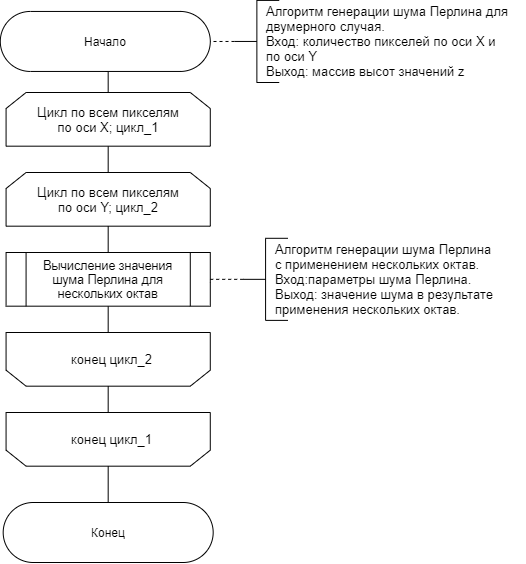
\includegraphics[scale=0.4]{../../../../../../../msys64/home/Лев/bmstu_cg_course_project/rpz/images/perlin_1}
		\caption{Градиенты на оси Ох}
		\label{png:perlin_1}
	}
\end{figure}

Если продолжить эти линии и опустить перпендикуляры из некоторых точек этих прямых к оси Ох, то получим следующую картину (рисунок \ref{png:perlin_2}).
\begin{figure}[H]
	\centering{
		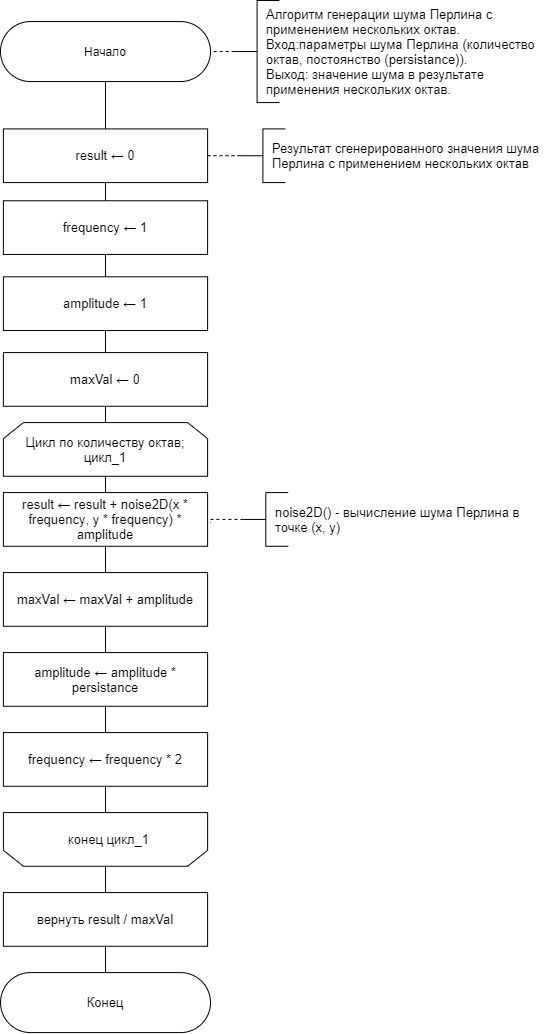
\includegraphics[scale=0.4]{../../../../../../../msys64/home/Лев/bmstu_cg_course_project/rpz/images/perlin_2}
		\caption{Перпендикуляры к оси Ох}
		\label{png:perlin_2}
	}
\end{figure}

Теперь нужно выяснить, как можно пары точек для каждого «х» представить в виде гладкой кривой. Для решения этой проблемы применяют функцию, называемую smoothstep. Применяется полином третьей степени по формуле (\ref{eq:ref1}):

\begin{equation}
	smoothstep(x) = 3x^2 - 2x^3
	\label{eq:ref1}
\end{equation}
 
Таким образом, выполнились необходимые условия: получен плавный переход между сегментами функции (производная в целочисленных значениях yна оси Ох равна нулю), а также альтернативу использования более сложных методов интерполяции. Следовательно, интерполируется не сам градиент, а его скалярное произведение на вектор от узла до точки. 

Спустя некоторое время Кен Перлин предлагает улучшенную версию функции $smoothstep$ по формуле (\ref{eq:ref2}), которая при $x = 0$ и $x = 1$ имеет нулевые производные первого и второго порядков:

\begin{equation}
	smoothstep(x) = 6x^5 - 15x^4 + 10x^3
	\label{eq:ref2}
\end{equation}

Эти две функции очень похожи (рисунок \ref{png:smooth_function}), но кривая пятой степени также имеет нулевую вторую производную в своих конечных точках, что делает функцию шума всюду непрерывной и более подходящей для общих задач компьютерной графики, связанных со смещением поверхности и отображением рельефа \cite{improved_perlin_noise}.

\begin{figure}[H]
	\centering{
		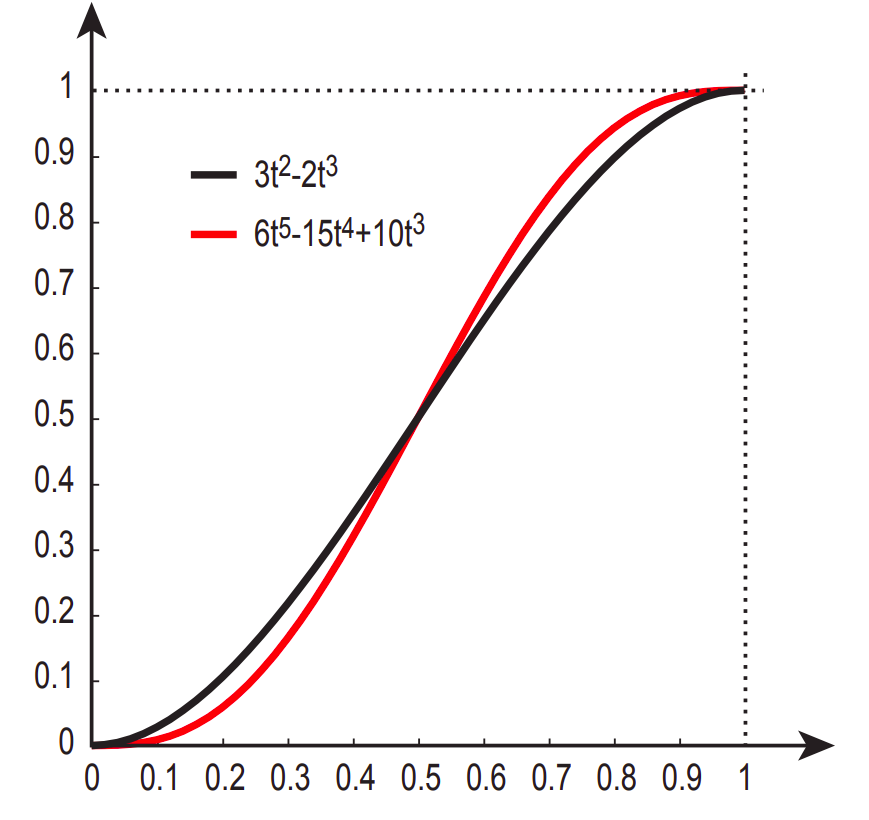
\includegraphics[scale=0.25]{../../../../../../../msys64/home/Лев/bmstu_cg_course_project/rpz/images/smooth_function}
		\caption{Шум Перлина}
		\label{png:smooth_function}
	}
\end{figure}

Для создания более органичного и интересного результата необходимо добавить несколько шумовых функций, называемых октавами. Каждая функция шума имеет частоту, в два раза большую чем предыдущая. Поэтому градиенты будут находиться в точках $(x = 0, 0.5, 1,..)$. Применив до 4-5 октав к исходной функции для одномерного измерения, получим следующую картину (рисунок \ref{png:octaves}).

\begin{figure}[H]
	\centering{
		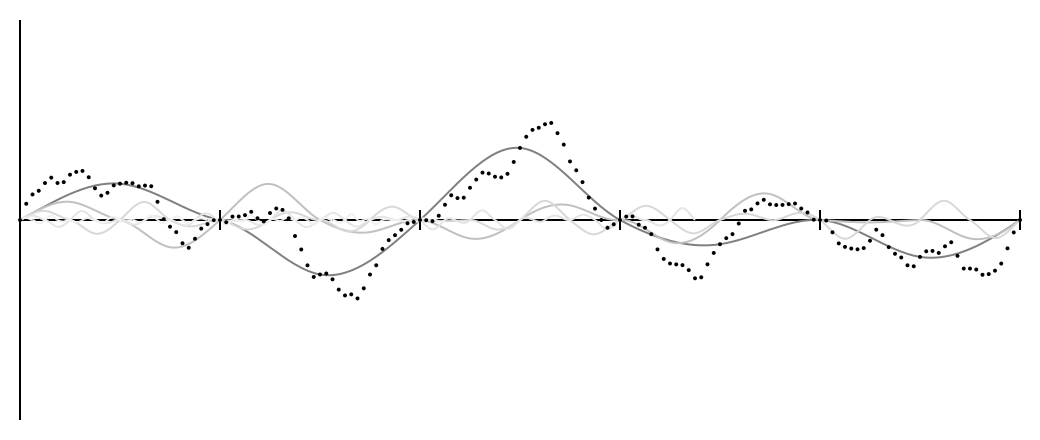
\includegraphics[scale=0.4]{../../../../../../../msys64/home/Лев/bmstu_cg_course_project/rpz/images/octaves}
		\caption{Результат наложения нескольких октав}
		\label{png:octaves}
	}
\end{figure}

Использование 2d-измерения:
Основное отличие от одномерного случая — целочисленные координатные точки определяют регулярную сетку (рисунок \ref{png:math_perlin_1}) \cite{math_perlin_noise}. В каждой точке выбирается псевдослучайный единичный вектор — градиент g, для которого важно только направление (рисунок \ref{png:math_perlin_2}). 

\begin{figure}[H]
	\centering{
		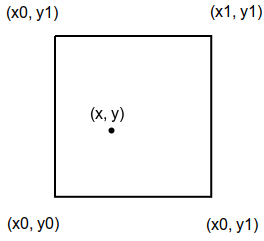
\includegraphics[scale=0.6]{../../../../../../../msys64/home/Лев/bmstu_cg_course_project/rpz/images/math_perlin_1}
		\caption{Регулярная сетка}
		\label{png:math_perlin_1}
	}
\end{figure}

\begin{figure}[H]
	\centering{
		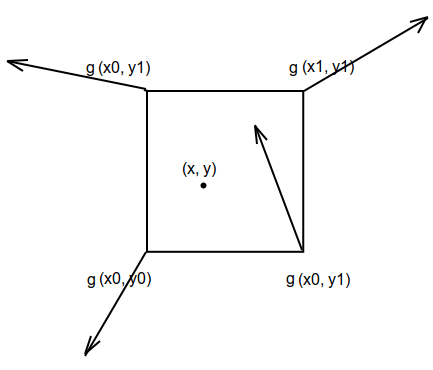
\includegraphics[scale=0.6]{../../../../../../../msys64/home/Лев/bmstu_cg_course_project/rpz/images/math_perlin_2}
		\caption{Псевдослучайные градиенты, связанные с узлами сетки}
		\label{png:math_perlin_2}
	}
\end{figure}

Градиент $g$ имеет вид случайности, но с важным учетом того, что он всегда возвращает один и тот же градиент для одной и той же точки сетки, каждый раз, когда он вычисляется. Также важно, чтобы у каждого направления были равные шансы быть выбранным. Для каждой точки сетки мы генерируем вектор, идущий от точки сетки до координат $(x, y)$, который легко вычисляется путем вычитания точки сетки из $(x, y)$ (рисунок \ref{png:math_perlin_3}).

\begin{figure}[H]
	\centering{
		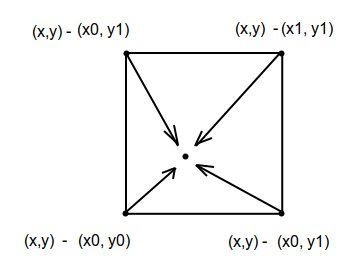
\includegraphics[scale=0.6]{../../../../../../../msys64/home/Лев/bmstu_cg_course_project/rpz/images/math_perlin_3}
		\caption{Векторы из узлов сетки до точки (x, y)}
		\label{png:math_perlin_3}
	}
\end{figure}

Расчет влияния каждого псевдослучайного градиента на конечный результат позволяет сгенерировать результат как средневзвешенное значение этих влияний. Для этого вычисляется скалярное произведение градиента и вектора, идущего от связанной с ним точки сетки к точке с координатами $(x, y)$ по формулам (\ref{eq:ref3}), (\ref{eq:ref4}), (\ref{eq:ref5}), (\ref{eq:ref6}):

\begin{equation}
	s = g(x_0, y_0) \cdot ((x, y) - (x_0, y_0))
	\label{eq:ref3}
\end{equation}
\begin{equation}
	t = g(x_1, y_0) \cdot ((x, y) - (x_1, y_0))
	\label{eq:ref4}
\end{equation}
\begin{equation}
	u = g(x_0, y_1) \cdot ((x, y ) - (x_0, y_1))
	\label{eq:ref5}
\end{equation}
\begin{equation}
	v = g(x_1, y_1) \cdot ((x, y) - (x_1, y_1))
	\label{eq:ref6}
\end{equation}

Результат применения формул (\ref{eq:ref3}), (\ref{eq:ref4}), (\ref{eq:ref5}), (\ref{eq:ref6}) показан на рисунке \ref{png:math_perlin_4}.
\begin{figure}[H]
	\centering{
		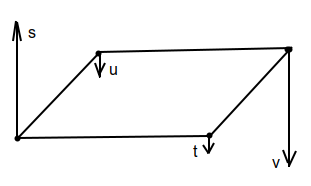
\includegraphics[scale=0.6]{../../../../../../../msys64/home/Лев/bmstu_cg_course_project/rpz/images/math_perlin_4}
		\caption{Влияние на узлы сетки}
		\label{png:math_perlin_4}
	}
\end{figure}

Затем выполняется нахождение средневзвешенного значения $s$ и $t$, построив билинейную функцию, которая отображает 0 в $s$ и 1 в $t$, и оценив ее по весу измерения $x$. Мы назовем это среднее значение $lerpa$. Выполним то же самое для $u$ и $v$ и запишем результат в $lerpb$. Математически можно рассчитать для точки P(x,y) по формулам (\ref{eq:ref7}), (\ref{eq:ref8}), (\ref{eq:ref9}), (\ref{eq:ref10}), (\ref{eq:ref11}), (\ref{eq:ref12}):
\begin{equation}
	fade = 6t^5 - 15t^4 + 10t^3
	\label{eq:ref7}
\end{equation}
\begin{equation}
	S_x = fade(x)
	\label{eq:ref8}
\end{equation}
\begin{equation}
	S_y = fade(y)
	\label{eq:ref9}
\end{equation}
\begin{equation}
	lerpa = s + S_{x} \cdot (t - s)
	\label{eq:ref10}
\end{equation}
\begin{equation}
	lerpb = u + S_x \cdot (v - u)
	\label{eq:ref11}
\end{equation}
\begin{equation}
	lerp = lerpa + sy(lerpb - lerpa)
	\label{eq:ref12}
\end{equation}

Теперь находится вес для измерения $y$, $S_y$, оценивая кривую сглаживания при $y - y_0$, и, наконец, берется взвешенная сумма $a$ и $b$, чтобы получить выходное значение $z$.

Применив для двумерного случая несколько октав, получим интересный результат (рисунок \ref{png:more_octaves}).
\begin{figure}[H]
	\captionsetup{justification=centering}
	\centering{
		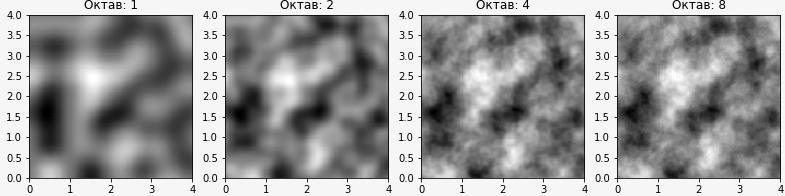
\includegraphics[scale=0.6]{../../../../../../../msys64/home/Лев/bmstu_cg_course_project/rpz/images/more_octaves}
		\caption{Изменение детализации шума Перлина с применением нескольких октав}
		\label{png:more_octaves}
	}
\end{figure}

\section{Алгоритмы удаления невидимых ребер и поверхностей}
\subsection{Алгоритм Варнока}
Алгоритм работает в пространстве изображения.

Основная идея данного алгоритма заключается в том, что исходный экран рассматривается как окно. Производится анализ этого окна: пусто ли его содержимое или оно достаточно для визуализации. Если это не так, то производится разбиение данного окна на подобласти (рисунок \ref{png:varnok}) до тех пор, пока информация, содержащаяся в нем, не станет достаточной для визуализации данного фрагмента. Если полученной информации достаточно, то происходит её усреднение и результат изображается одинаковым цветом или интенсивностью. Для эффективной работы данного алгоритма требуется выбрать наиболее подходящий способ разбиения окна, тем самым усложнив способ и критерий разбиения. Для растрового дисплея на экране пределом деления окна является один пиксель - в случае простого алгоритма. Единой версии данного алгоритма не существует, существует только его различные модификации.

\begin{figure}[H]
	\centering{
		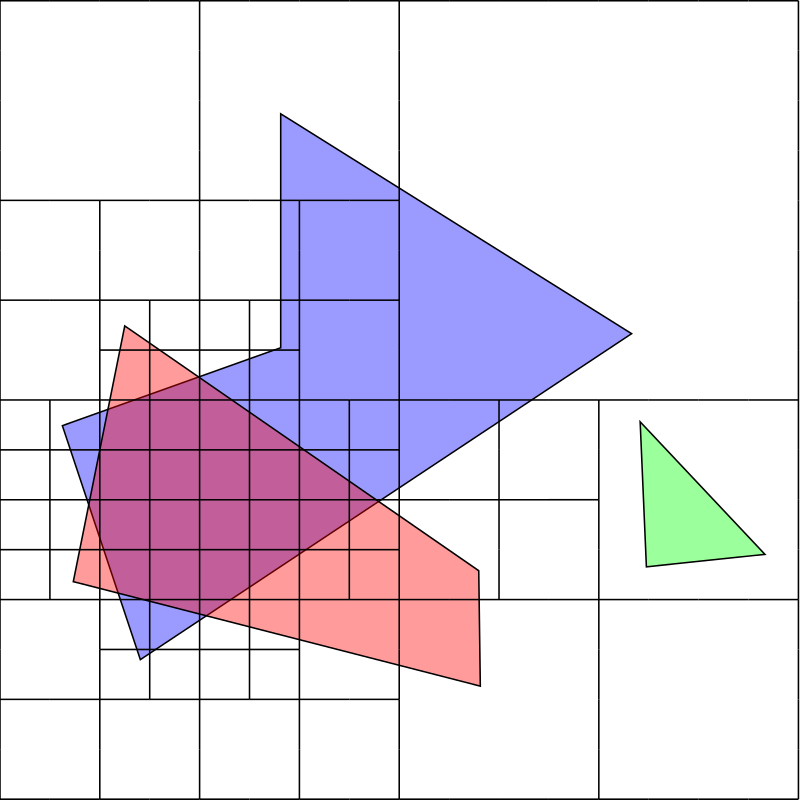
\includegraphics[scale=0.3]{../../../../../../../msys64/home/Лев/bmstu_cg_course_project/rpz/images/varnok}
		\caption{Разбиение окна на подобласти}
		\label{png:varnok}
	}
\end{figure}

К недостатку данного алгоритма относится следующее: при увеличении сложности сцены число разбиений может так увеличиться, что приведет к снижению временной эффективности работы программы.

\subsection{Алгоритм Z-буфера}
Алгоритм работает в пространстве изображения.

Основная идея данного алгоритма — использование буфера глубины каждого видимого пикселя изображения сцены \cite{zbuffer}. Для каждого объекта сцены сравнивается значение координаты $z$ с буфером глубины, который изначально заполняется значением, соответствующим максимальному. Если рассматриваемый пиксель находится ближе пикселя, который находится в буфере кадра, то производится корректировка, и этот пиксель заносится в этот буфер. Используется также и другой буфер, который запоминает цвет пикселя изображения. Если сцена подвергается видовому преобразованию и отсекается до фиксированного диапазона координат z значений, то можно использовать z-буфер с фиксированной точностью. Информацию о глубине нужно обрабатывать с большей точностью, чем координатную информацию на плоскости $(x, y)$; обычно бывает достаточно 20 бит.

Преимущества:
\begin{itemize}
	\item позволяет работать со сложными объектами сцены — позволит достаточно легко выполнить визуализацию пересечения сложных поверхностей;
	\item объекты сцены могут заноситься в произвольном порядке — не нужно выполнять предварительную сортировку по глубине, что позволит сделать выигрыш по производительности;
	\item сцена может обрабатываться любого размера — вычислительная сложность не более чем O(n) — необходимо для быстрого рендеринга;
	\item буферы кадра и глубины вместе занимают памяти (буфер кадра размером 1920 $\times$ 1080 $\times$ 24 бит в комбинации с z-буфером размером 1920 $\times$ 1080 $\times$ 20 бит требует около 11 Мб), что по сегодняшним темпам развития технологий не является критичным. 
\end{itemize}

К недостаткам относится возникновение трудностей реализации эффектов прозрачности и просвечивания, а также устранение лестничного эффекта.

\subsection{Алгоритм обратной трассировки лучей}
Данный алгоритм работает в пространстве изображения.

В этом алгоритме происходит отслеживание лучей не от источников света, а наоборот, от точки наблюдателя — в обратном направлении (рисунок \ref{png:ray_tracing}). При формировании конечного изображения учитываются только те лучи, которые вносят вклад в его формирование. То есть чтобы определить цвет пикселя экрана, необходимо из камеры провести луч и найти ближайшую точку пересечения со сценой, в которой и определяется освещенность этой точки. Она получается в результате сложения энергии отраженного и преломленного, которые получены непосредственно от источников света и также от других объектов сцены. В результат конечного изображения также учитывается и ослабление света, проходящий через прозрачный материал.

\begin{figure}[H]
	\centering{
		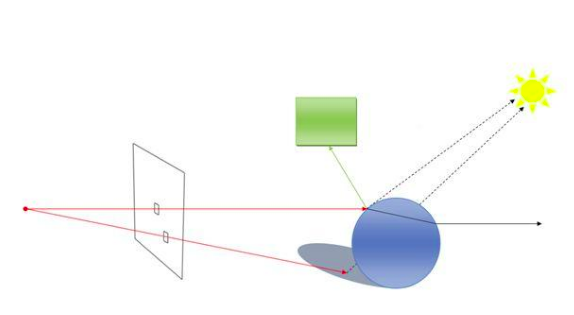
\includegraphics[scale=0.5]{../../../../../../../msys64/home/Лев/bmstu_cg_course_project/rpz/images/ray_tracing}
		\caption{Обратная трассировка лучей}
		\label{png:ray_tracing}
	}
\end{figure}

Преимущества:
\begin{itemize}
	\item позволяет получить сложные изображения, использующие законы геометрической оптики (преломление, отражение, тени);
	\item можно выполнить распараллеливание вычислений.
\end{itemize}

Недостатки:
\begin{itemize}
	\item является одним из самых медленных алгоритмов синтеза изображений по сравнению с остальными.
\end{itemize}

\section{Модель освещения}
При работе с изображением для реалистичности необходимо также учитывать немало важный компонент — свет, который позволяет рассмотреть исходную модель более детально. Для этих целей существует модель освещения — выполнение расчетов интенсивности отраженного к наблюдателю света в каждом пикселе изображения.

Различают несколько видов модели освещения.
\begin{enumerate}
	\item Локальная — в ней учитывается тот свет, который попал в рассматриваемую точку от источника света.
	\item Глобальная — учитывает все свойства локального света, а также свет от других объектов, отраженный или пропущенный. Используя это, можно воспроизводить такие эффекты как преломление (прозрачность, полупрозрачность), отражение и затенение.
\end{enumerate}

Существует несколько моделей освещенности, которые до сих пор пользуются популярностью и используются в современных программах: модель Ламберта и модель Фонга. Пусть заданы точечный источник света, расположенный в некоторой точке, поверхность, которая будет освещаться и наблюдатель. Будем считать, что наблюдатель точечный. Каждая точка поверхности имеет свои координаты, и в ней определена нормаль к поверхности. Для удобства все векторы, описанные ниже, берутся единичными. В этом случае косинус угла между ними совпадает со скалярным произведением.

\subsection{Модель освещения Ламберта}
Такое освещение называют диффузным, и его смысл заключается в том, что падающий свет отражается во всех направлениях (рисунок \ref{png:lambert_light_model}) \cite{lambert_light_model}.
\begin{figure}[H]
	\centering{
		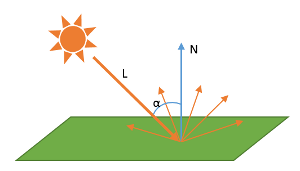
\includegraphics[scale=0.9]{../../../../../../../msys64/home/Лев/bmstu_cg_course_project/rpz/images/lambert_light_model}
		\caption{Модель освещения Ламберта}
		\label{png:lambert_light_model}
	}
\end{figure}

Освещение рассчитывается по формуле (\ref{eq:lambert}):
\begin{equation}
	I = (\overline{N}, \overline{L}) = \overline{N} \cdot \overline{L},
	\label{eq:lambert}
\end{equation}

где $\overline{N}$ - вектор нормали к поверхности в точке, $\overline{L}$ - падающий на точку луч света.


\subsection{Модель освещения Фонга}
Освещенность такой модели складывается из трех компонент: фоновое освещение, рассеянный свет и бликовая составляющая (рисунок \ref{png:phong_light_model}). Свойства источника определяют мощность излучения для каждой из этих компонент, а свойства материала поверхности определяют её способность воспринимать каждый вид освещения.
\begin{figure}[H]
	\centering{
		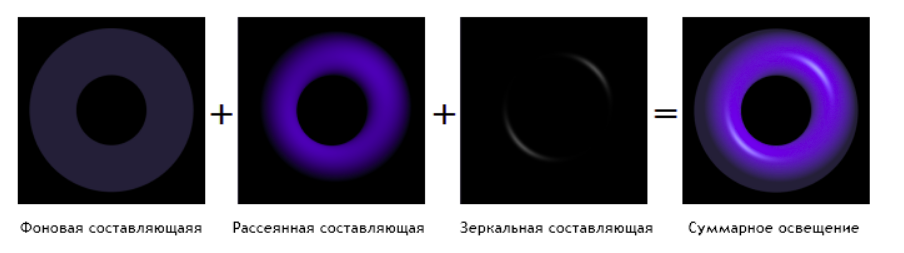
\includegraphics[scale=0.5]{../../../../../../../msys64/home/Лев/bmstu_cg_course_project/rpz/images/phong_light_model}
		\caption{Модель освещения Фонга}
		\label{png:phong_light_model}
	}
\end{figure}

Освещение рассчитывается по формуле (\ref{eq:phong}):
\begin{equation}
	I = k_{\alpha} \cdot i_\alpha + k_d \cdot (\overline{N}, \overline{L}) + k_s \cdot (\overline{R}, \overline{V})^\rho,
	\label{eq:phong}
\end{equation}
где $\overline{N}$ - вектор нормали к поверхности в точке, $\overline{L}$ - падающий на точку луч света, $\overline{R}$ - отраженный луч, $\overline{V}$ - вектор, направленный к наблюдателю, $k_\alpha, k_d, k_s$ - коэффициенты фонового, диффузного и зеркального освещения соответственно; $\rho$ - степень, аппроксимирующая пространственное распределение зеркально отраженного света. По сравнению с простой моделью освещения модель освещения Фонга обеспечивает большую реалистичность, но при этому требует больше вычислений.

\section{Алгоритмы закраски}
\subsection{Простая закраска}
Суть данного алгоритма заключается в том, что для каждой грани объекта находится вектор нормали, и с его помощью в соответствии с выбранной моделью освещения вычисляется значение интенсивности, с которой закрашивается вся грань.

Данный метод закраски обладает большим быстродействием по сравнению с другими методами, однако все пиксели грани имеют одинаковую интенсивность - сцена выглядит недостаточно реалистично.

\subsection{Закраска по Гуро}
В этом методе выполняется вычисление цвета модели для каждого пикселя\cite{guro_shading}. Данный метод отличается от простой закраски тем, что разные точки грани закрашиваются при помощи  разных значений интенсивности. Для это в каждой вершине грани находится усредненный вектор нормали всех плоскостей, в которых принадлежит эта вершина, и в них вычисляется значение интенсивности. Затем найденные значения интенсивности билинейно интерполируются по всем точкам грани (рисунок \ref{png:guro_interolation_light}). При помощи такого алгоритма получится сглаженное изображение.

\begin{figure}[H]
	\centering{
		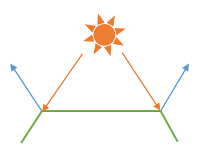
\includegraphics[scale=1]{../../../../../../../msys64/home/Лев/bmstu_cg_course_project/rpz/images/guro_interolation_light}
		\caption{Интерполяция интенсивностей закраски по Гуро}
		\label{png:guro_interolation_light}
	}
\end{figure}

Недостатком такой интерполяции является блик как на рисунке \ref{png:guro_blick}, который будет правильно отрисован в вершине многоугольника, но неестественно распространен по соседним полигонам с помощью такого метода интерполяции.

\begin{figure}[H]
	\centering{
		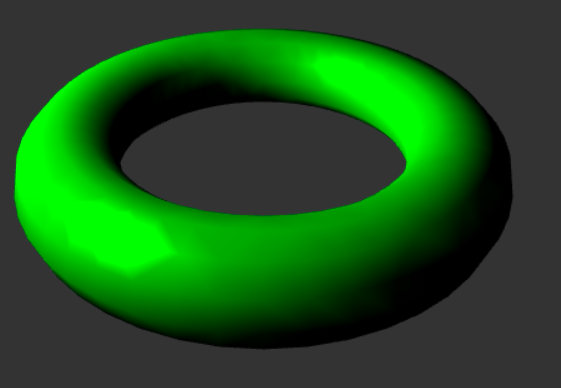
\includegraphics[scale=0.4]{../../../../../../../msys64/home/Лев/bmstu_cg_course_project/rpz/images/guro_blick}
		\caption{Появление неестественного блика}
		\label{png:guro_blick}
	}
\end{figure}

\subsection{Закраска по Фонгу}
При таком подходе выполняется билинейная интерполяция не цвета, а нормали (рисунок \ref{png:phong_interolation_light}). При таком подходе изображение получается более качественным, и исчезает проблема с бликами (рисунок \ref{png:phong_blick}). Но для достижения такого результата требуется больше вычислительных ресурсов — понижается скорость работы по сравнению с моделью Гуро. Из-за увеличения разрешения данный метод применятся в современных видеокартах при отрисовке изображения.

\begin{figure}[H]
	\centering{
		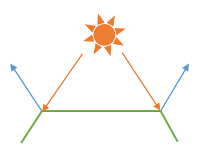
\includegraphics[scale=1]{../../../../../../../msys64/home/Лев/bmstu_cg_course_project/rpz/images/guro_interolation_light}
		\caption{Интерполяция нормалей закраски по Фонгу}
		\label{png:phong_interolation_light}
	}
\end{figure}

\begin{figure}[H]
	\centering{
		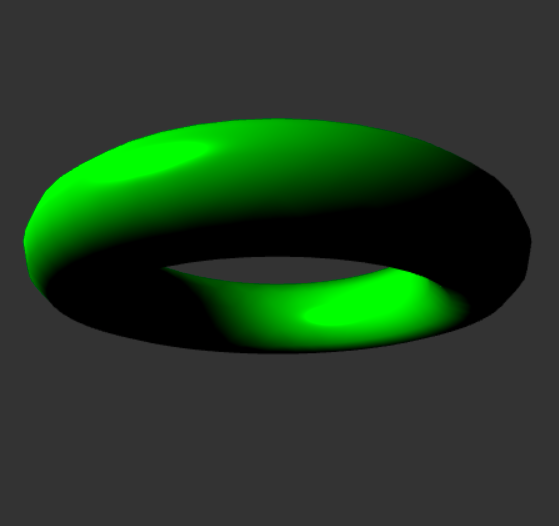
\includegraphics[scale=0.4]{../../../../../../../msys64/home/Лев/bmstu_cg_course_project/rpz/images/phong_shading}
		\caption{Пример блика закраски Фонга}
		\label{png:phong_blick}
	}
\end{figure}

\section{Вывод}
В данном разделе был произведен анализ существующих методов, необходимых для построения и визуализации трехмерного ландшафта. Выбранный способ представления данных о трехмерном ландшафте — карта высот. Наряду с использованием шума Перлина будет использован алгоритм z-буфера. В качестве освещения выбрана модель Ламберта и модель интерполяции света по Гуро — в совокупности они приведут к качественному результату. Так как важна скорость отрисовки изображения на экране, то были выбраны именно данные алгоритмы.

На вход программе будут подаваться параметры шума Перлина, которые позволяют выводить различный вид ландшафта. Пользователю будет доступно изменять эти параметры, выполнять поворот и масштабирование сцены, а также увеличение размера исходной сцены. Возможно изменение положения точечного источника света. В результате программа должна выдавать сгенерированный трехмерный ландшафт. Программа должна корректно реагировать на действия пользователя.